\documentclass[a4paper,11pt]{article}

% ====================
% PACKAGES DE BASE
% ====================
\usepackage[utf8]{inputenc}
\usepackage[T1]{fontenc}
\usepackage[french]{babel}
\usepackage{amsmath, amssymb, amsfonts}
\usepackage{graphicx}
\usepackage{geometry}
\usepackage{hyperref}
\usepackage{booktabs}
\usepackage{float}
\usepackage{xcolor}
\usepackage{caption}
\usepackage{subcaption}
\usepackage{siunitx}

% ====================
% MISE EN PAGE
% ====================
\geometry{margin=2.5cm}
\setlength{\parskip}{6pt}
\setlength{\parindent}{0pt}
\hypersetup{
    colorlinks=true,
    linkcolor=blue,
    urlcolor=blue,
    citecolor=blue
}

% ====================
% INFORMATIONS DU DOCUMENT
% ====================
\title{\textbf{Compte rendu du TP2}\\[4pt]
\large Modélisation de la distance moyenne au plus proche voisin (DMPPV)}
\author{Groupe : \textit{Maël Verbois, Jules Onée, Reyen Selmi} \\[2pt] Cours : ROB}


% ====================
% DOCUMENT
% ====================
\begin{document}

\maketitle


% ====================
% INTRODUCTION
% ====================
\section{Compte Rendu}
L’objectif de ce travail est de modéliser et de résoudre le problème d'optimisation combinatoire associé à la fragmentation
du paysage. L'indicateur utilisé pour la mesure de la fragmentation est la distance moyenne au plus proche voisin (DMPPV).
On modélisera le problème sous la forme d'un problème d'optimisation combinatoire fractionnaire avec pour fonction objectif une 
fraction rationelle. On résoudra ce problème à l'aide de l'algorithme de Dinkelbach implémentée en Julia en utilisant Gurobi comme solveur de PLNE.
Finalement on étudiera le complexité temporelle sur des instances de tailles variables.

% ====================
% QUESTION i
% ====================

\subsection*{Question 1 -  Modéliser le problème de la sélection d'un ensemble de parcelles d'aire totale comprise
entre Amin et Amax, de coût total inférieur ou égal à B et qui minimise dmppv.
}

On cherche à modéliser le problème de sélection d’un ensemble de parcelles de sorte que :
\begin{itemize}
    \item l’aire totale des parcelles sélectionnées soit comprise entre $A_{\min}$ et $A_{\max}$,
    \item le coût total ne dépasse pas un budget $B$,
    \item et la distance moyenne au plus proche voisin (dmppv) soit minimisée.
\end{itemize}

On introduit pour cela les variables binaires de décision :
\[
s_{ij} =
\begin{cases}
1 & \text{si la parcelle } (i,j) \text{ est sélectionnée,}\\
0 & \text{sinon.}
\end{cases}
\]

On note :
\begin{itemize}
    \item $c_{ij}$ : le coût associé à la parcelle $(i,j)$.
\end{itemize}


La fonction objectif vise à minimiser la distance moyenne au plus proche voisin (DMPPV), qui sera définie dans la question suivante. Le modèle général s’écrit donc :
\[
\begin{aligned}
\min \quad & DMPPV(s) \\
\text{sous contraintes} \quad &
\begin{cases}
A_{\min} \leq \displaystyle\sum_{i,j} a_{ij} s_{ij} \leq A_{\max},\\[8pt]
\displaystyle\sum_{i,j} c_{ij} s_{ij} \leq B,\\[8pt]
s_{ij} \in \{0,1\}, \quad \forall (i,j).
\end{cases}
\end{aligned}
\]

% ====================
% QUESTION ii
% ====================
\subsection{Question 2 -  Écrire le modèle sous la forme d'un programme d'optimisation combinatoire fractionnaire, où les fractions sont des ratios de deux fonctions linéaires.}

On a facilement par la définition
\[
DMPPV =
\frac{1}{\sum_{i,j} s_{ij}} 
\cdot 
\sum_{i,j} 
\min \left\{ d_{(i,j),(k,l)} \;\big|\; (i,j) \neq (k,l) \right\}, 
\]
\[
\text{avec $d_{(i,j),(k,l)}$ la distance euclidienne entre la parcelle $(i,j)$ et la parcelle $(k,l)$.}
\]
La difficulté réside dans l'expression de la distance du voisin le plus proche d'une parcelle $s_{ij}$.
Pour exprimer cette quantité comme une fonction linéaire on introduit : 
\begin{itemize}
    \item $d(i, j, k, l)$ la distance entre la parcelle $(i,j)$ et la parcelle $(k,l)$
    \item { $ 
    m(i, j, k, l) = 
    \begin{cases}
        1 & \shortstack[l]{si les parcelles $(i,j),(k,l)$ sont leurs voisines les plus \\ proches respectives} \\
        0 & \text{sinon.}
    \end{cases}
        $
    }
\end{itemize}
Ce qui nous donne l'expression suivante 

\[
    DMPPV = \frac{1}{\sum_{i,j} s_{ij}} 
    \cdot 
    \sum_{i,j,k,l \;\big|\; (i,j) \neq (k,l)} m(i,j,k,l) \cdot d(i,j,k,l) 
\]

Il faut aussi modéliser les contraintes suivantes pour garantir les propriétés des $m(i,j,kl)$
\begin{itemize}
    \item Chaque parcelle $(i,j)$ n'a qu'un seul voisin considéré comme le plus proche pour éviter les doubles comptages
    \item Deux parcelles $(i,j)$ et $(k,l)$ ne peuvent être considérées comme plus proches que si elles sont sélectionnée
\end{itemize}
Finalement, on obtient le modèle global suivant : 

\[
\begin{aligned}
\min \quad & DMPPV(s,m) =
\frac{
\displaystyle\sum_{i,j,k,l \;\big|\; (i,j) \neq (k,l)} m(i,j,k,l) \cdot d(i,j,k,l)
}{
\displaystyle\sum_{i,j} s_{ij}
} \\[4pt]
\text{sous contraintes} \quad &
\begin{cases}
A_{\min} \leq \displaystyle\sum_{i,j}  s_{ij} \leq A_{\max},\\[4pt]
\displaystyle\sum_{i,j} c_{ij} s_{ij} \leq B,\\[4pt]
\sum_{k,l \;\big|\; (i,j) \neq (k,l)} m(i,j,k,l) = 1, \quad \forall (i,j),\\[2pt]
m(i,j,k,l) \leq s_{ij}, \quad m(i,j,k,l) \leq s_{k,l}, \quad \forall (i,j) \neq (k,l),\\[2pt]
s_{ij} \in \{0,1\}, \quad \forall (i,j),\\
m(i,j,k,l) \in \{0,1\}, \quad \forall (i,j) \neq (k,l)
\end{cases}
\end{aligned}
\]
% ====================
% QUESTION iii
% ====================
\subsection{Question 3 - Résoudre l'instance présentée ci-dessous par l'algorithme de Dinkelbach / Question 4 : Pour chacune des 3 instances, donner le temps de calcul total, le nombre total de noeuds
développés dans l'arbre de recherche, le nombre d'itérations de l'algorithme de Dinkelbach, la valeur de la solution (valeur de dmppv) et les parcelles retenues.
}

On obtient les résultats suivants pour les 3 instances du sujet : 

\begin{figure}[H]
  \centering
  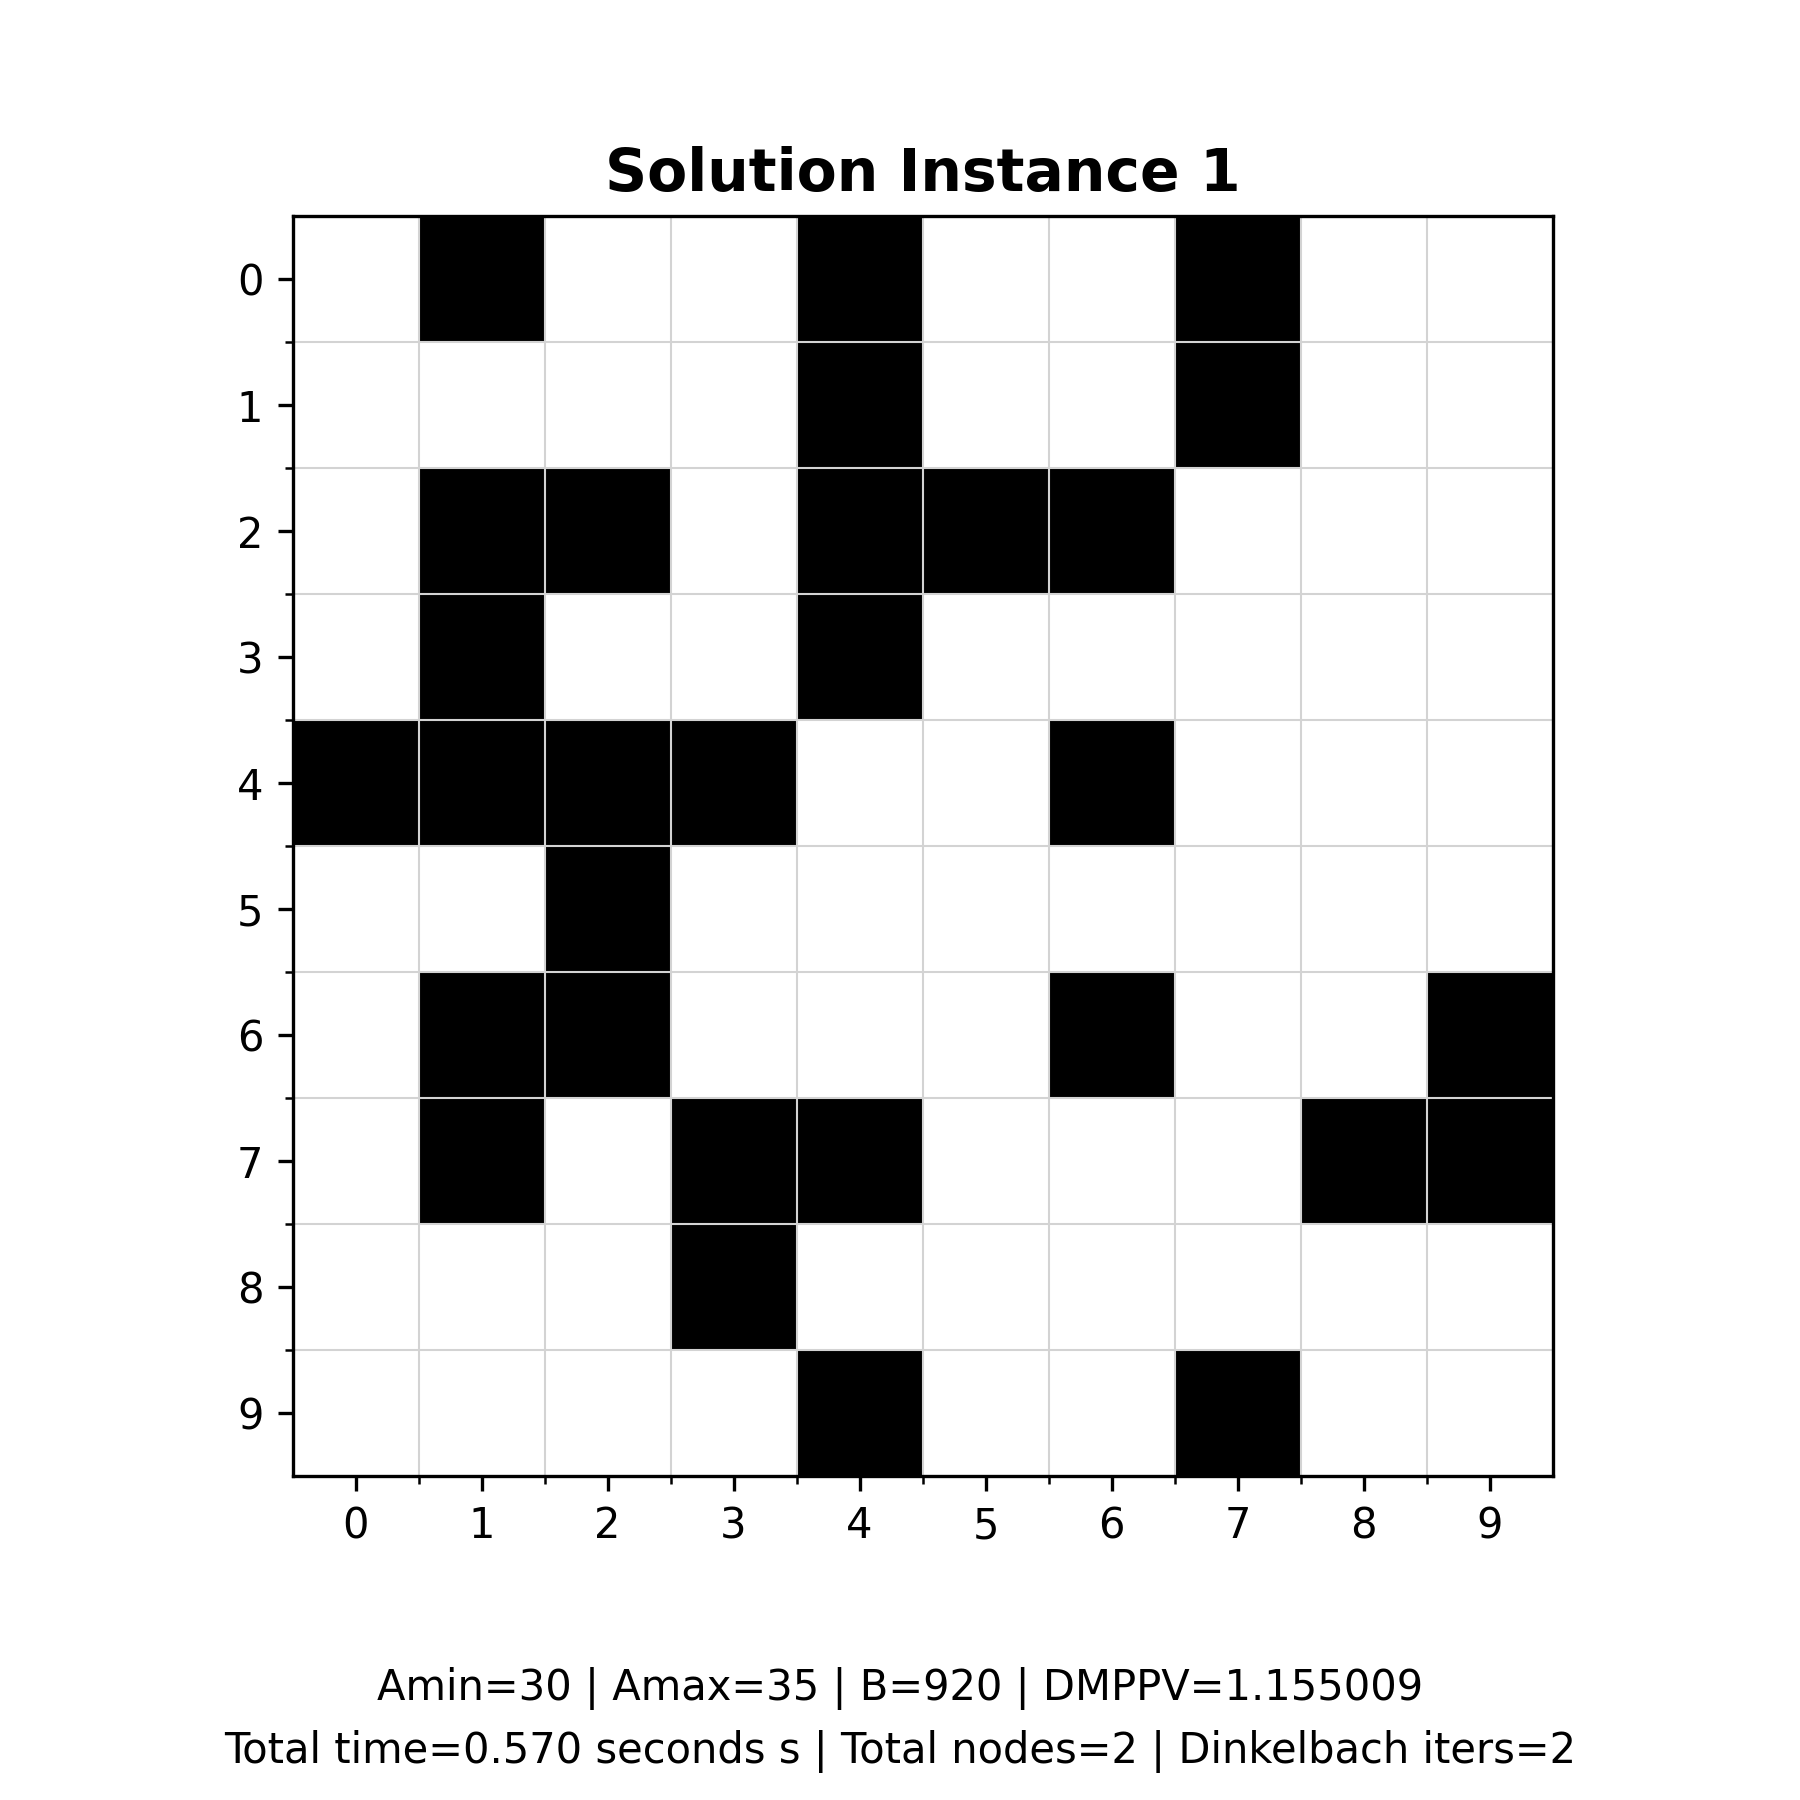
\includegraphics[width=0.7\textwidth]{figs/solution1_output.png}
\end{figure}

\begin{figure}[H]
  \centering
  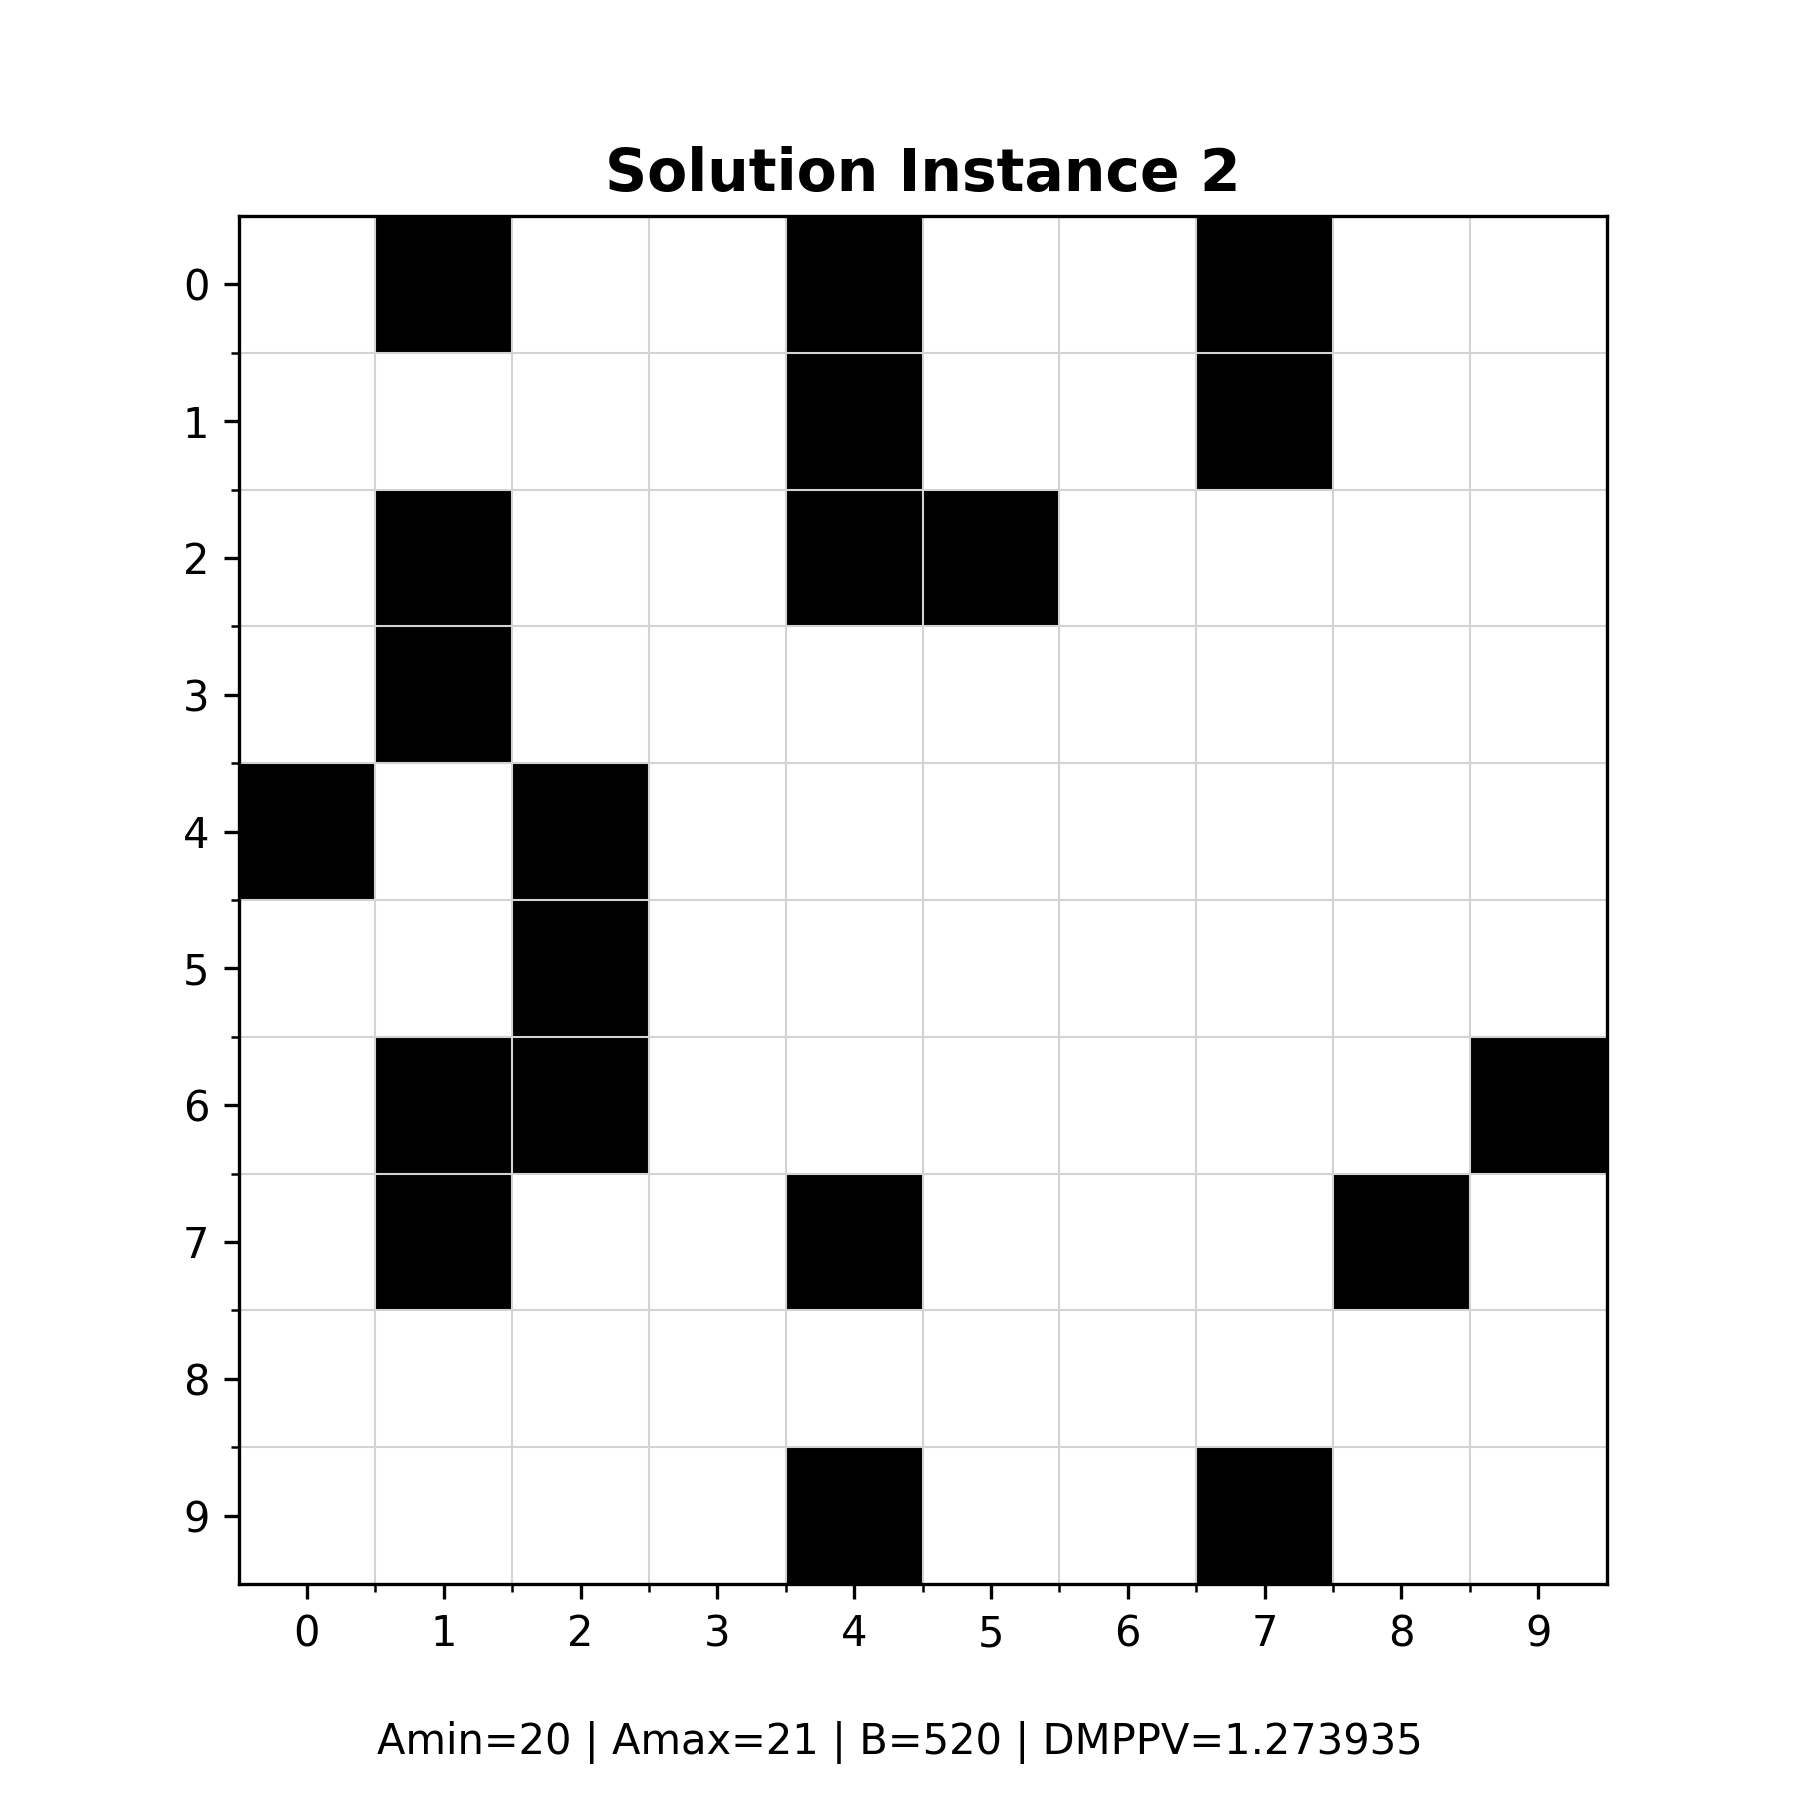
\includegraphics[width=0.7\textwidth]{figs/solution2_output.png}
\end{figure}

\begin{figure}[H]
  \centering
  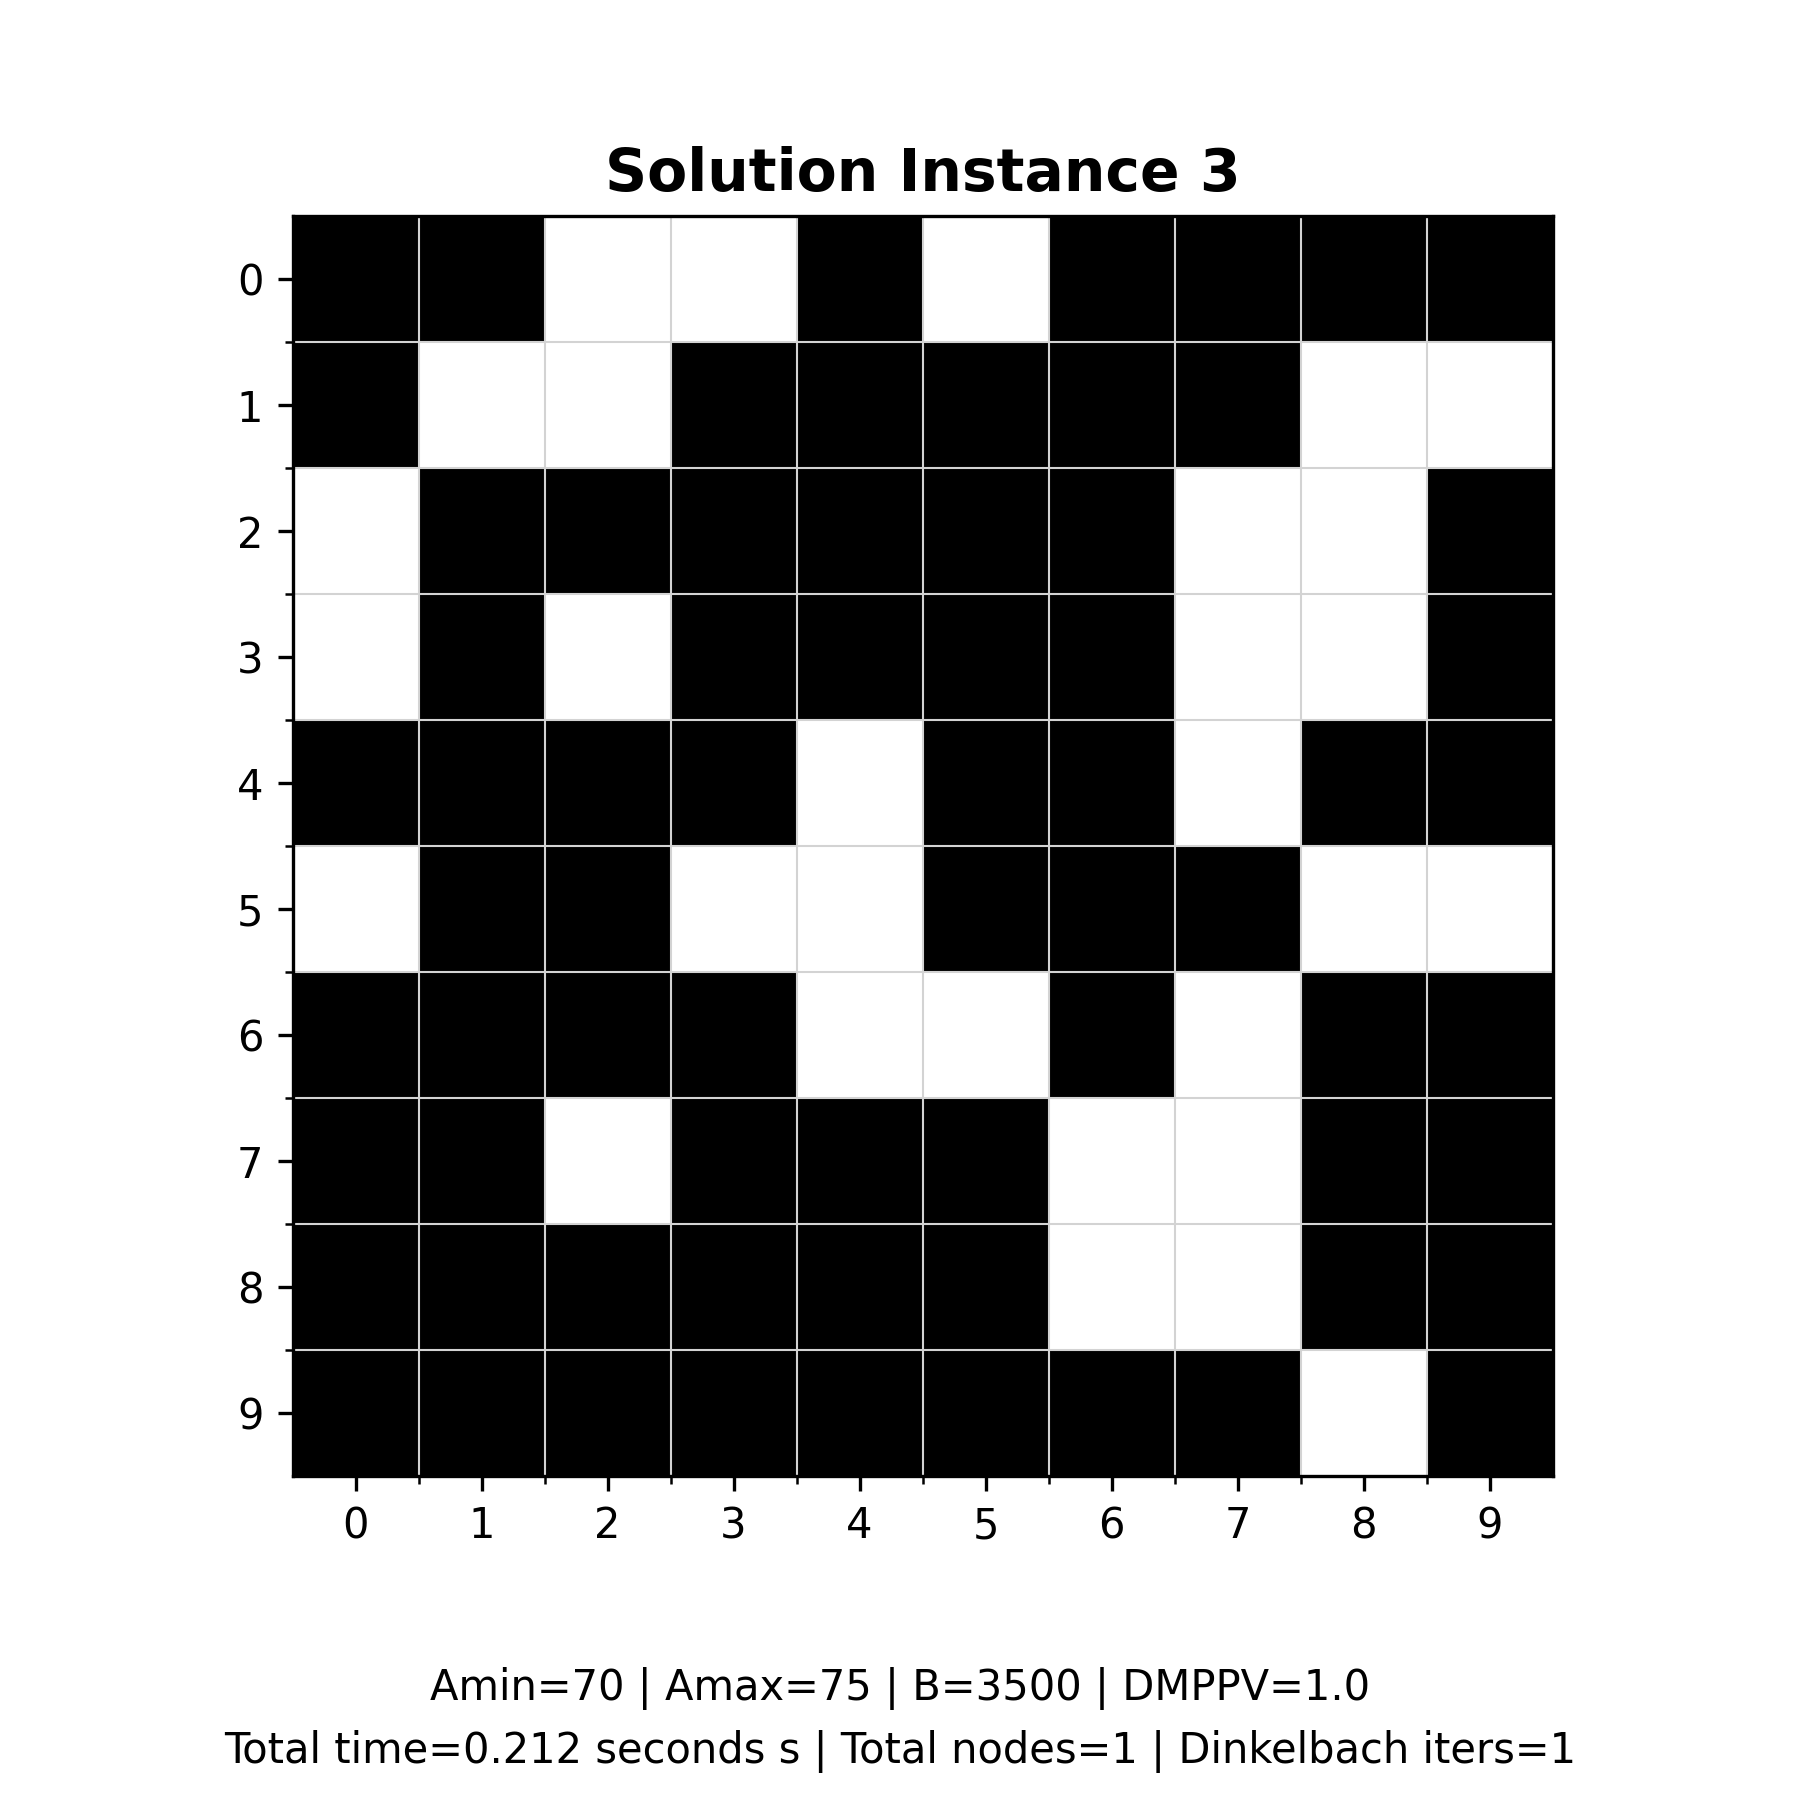
\includegraphics[width=0.7\textwidth]{figs/solution3_output.png}
\end{figure}

\subsection{Question 5 - Étudier le comportement de la méthode proposée en fonction de la taille des instances.
Pour cela, on engendrera aléatoirement des jeux d'essai}

Afin d'engendrer des instances aléatoires, on fait quelques hypothèses sur notre génération : 


On définit trois paramètres pour l'instance : 
\begin{itemize}
    \item Soit $n$ la dimension de la matrice des coûts $C = (c_{ij}) \in \mathbb{Z}^{n \times n}$, générée aléatoirement avec des valeurs multiples de 10 tirées uniformément entre 10 et $n^2$.  
    \item $A_{\min}$ : nombre minimal d'éléments sélectionnés, choisi uniformément dans l'intervalle $[\alpha n^2, \beta n^2]$,
    \item $A_{\max}$ : nombre maximal d'éléments sélectionnés, défini comme $A_{\max} = A_{\min} + \delta$, avec $\delta$ uniforme dans $[0, \gamma n^2]$,
    \item $B$ : somme sur un sous-ensemble de $A_{\min}$ éléments choisis uniformément dans $C$.
\end{itemize}

\subsection*{Valeurs par défaut des coefficients}
Les coefficients par défaut sont :
\[
\alpha = 0.3, \quad
\beta = 0.6, \quad
\gamma = 0.1
\]
Ils permettent de contrôler la cohérence de l'instance :
\begin{itemize}
    \item $\alpha$ et $\beta$ définissent la plage de $A_{\min}$, assurant que le nombre minimal d'éléments sélectionnés est proportionnel à $n^2$,
    \item $\gamma$ contrôle la variation possible entre $A_{\min}$ et $A_{\max}$,
\end{itemize}

La génération de l'instance garantit ainsi que :
\[
A_{\min} \leq |S| \leq A_{\max}, \quad \sum_{(i,j) \in S} c_{ij} = B
\]
pour un sous-ensemble $S$ de la matrice $C$.

\subsection{ Exemple d'instance générée aléatoirement}


\[
C =
\begin{bmatrix}
20 & 20 & 30 & 30 & 50 & 20 & 70 & 70 & 40 & 70\\
10 & 20 & 80 & 70 & 40 & 60 & 10 & 70 & 70 & 100\\
10 & 100 & 40 & 70 & 90 & 40 & 90 & 30 & 10 & 20\\
90 & 60 & 50 & 40 & 60 & 20 & 70 & 80 & 80 & 70\\
20 & 50 & 70 & 60 & 20 & 70 & 80 & 100 & 100 & 30\\
70 & 20 & 80 & 10 & 80 & 90 & 90 & 70 & 90 & 100\\
80 & 40 & 70 & 40 & 60 & 20 & 90 & 80 & 30 & 90\\
60 & 10 & 40 & 30 & 50 & 100 & 100 & 40 & 100 & 20\\
90 & 20 & 40 & 80 & 70 & 20 & 30 & 50 & 80 & 70\\
80 & 30 & 80 & 10 & 100 & 80 & 100 & 90 & 20 & 60
\end{bmatrix}
\]

avec les paramètres :

\[
A_{\min} = 44, \quad
A_{\max} = 53, \quad
B = 1437, \quad
n = 10
\]

En lançant l'algorithme sur des instances de taille 10 à 30 (3 fois par instance puis en faisant la moyenne des temps), 
On obtient le graphe de complexité temporelle suivant :

\begin{figure}[H]
  \centering
  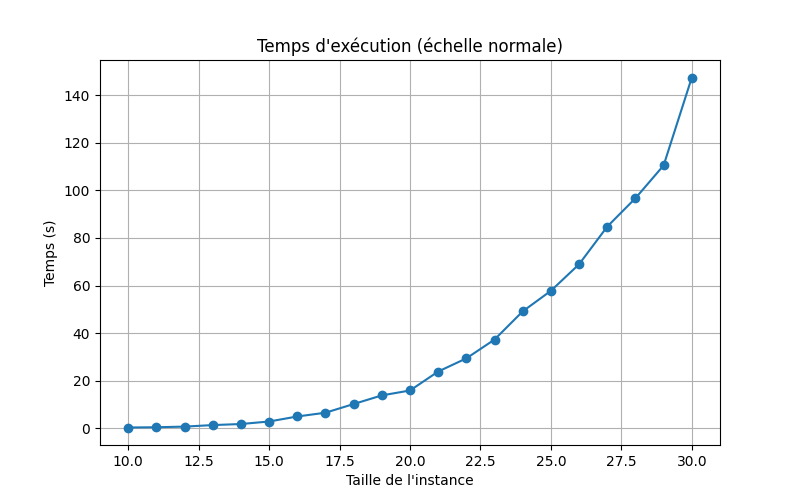
\includegraphics[width=0.7\textwidth]{figs/temps_execution_lineaire.png}
\end{figure}
\begin{figure}[H]
  \centering
  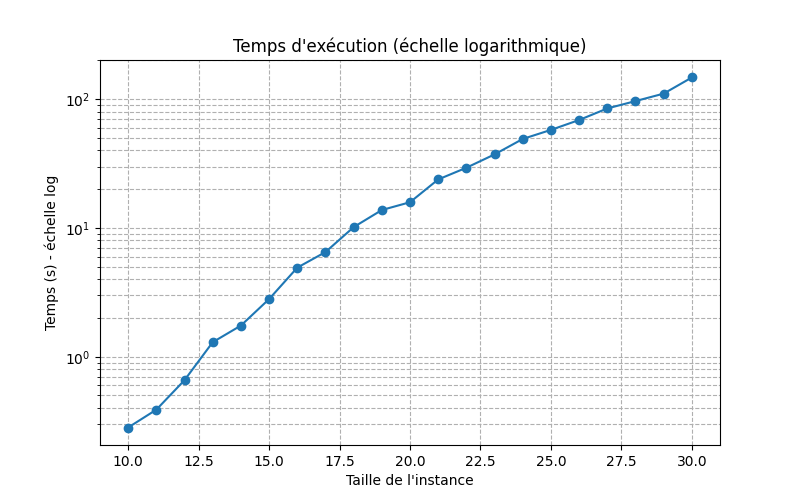
\includegraphics[width=0.7\textwidth]{figs/temps_execution_log.png}
\end{figure}

On remarque donc que même avec la spécificité de l'instance, 
la complexité temporelle reste exponentielle
% ====================
% CONCLUSION
% ====================

\end{document}
